%..............................................................................
% NOTE THAT THE graphicx PACKAGE HAS TO BE CALLED BEFORE \define@key
% OR CALLED AS \RequirePackage{keyval}
%\usepackage{graphicx}

\makeatletter
\RequirePackage{keyval}
\define@key{headers}{author}{\def\Author{#1}}
\define@key{headers}{title}{\def\Title{#1}}
\define@key{headers}{major}{\def\Major{#1}}
\define@key{headers}{mentor}{\def\Mentor{#1}}
\define@key{headers}{member}{\def\Member{#1}}


\usepackage{multicol}
\columnsep 0.25in
\newcommand{\SingleCol}{\section*{}}
\newcommand{\DoubleCols}{\begin{multicols*}{2}}
\newcommand{\TripleCols}{\begin{multicols*}{3}}
\newcommand{\QuadCols}{\begin{multicols*}{4}}
\newcommand{\EndCols}{\end{multicols*}}
\newcommand{\DoubleCol}{\begin{multicols}{2}}
\newcommand{\TripleCol}{\begin{multicols}{3}}
\newcommand{\QuadCol}{\begin{multicols}{4}}
\newcommand{\EndCol}{\end{multicols}}
\doublehyphendemerits=40000
\lefthyphenmin2
\righthyphenmin2

% CONFIGURE Figure and Table ENVIRONMENT FOR multicol
\newenvironment{Figure}
  {\par\medskip\noindent\minipage{\linewidth}}
  {\endminipage\par\medskip}
\newenvironment{Table}
  {\par\medskip\noindent\minipage{\linewidth}}
  {\endminipage\par\medskip}
%

% SET FONT SIZES
\newcommand{\hfn}{\usefont{T1}{ptm}{m}{n}\fontsize{12.0}{14.0}\selectfont}
\newcommand{\hfnl}{\usefont{T1}{ptm}{m}{n}\fontsize{16.8}{22.8}\selectfont}
\newcommand{\hfs}{\usefont{T1}{ptm}{m}{n}\fontsize{9.0}{9.8}\selectfont}

% SET VERTICAL SPACE
\newcommand{\Strut}[1]{\rule{0cm}{{#1}\textwidth}}
\usepackage{wrapfig}

% FIGURE FOR END OF DOCUMENT
\newcommand{\Next}{\\[0.48em]}
\newcommand{\portrait}[5]{
\setlength{\unitlength}{1cm}
\hspace*{-1.4cm}
\begin{tabular}{ll}
\hspace*{4.0cm} &  \\
\begin{picture}(0.0,0.0)({#1},{#2})
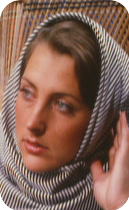
\includegraphics[scale={#3}]{./photos/portrait.png}
\end{picture} &
\parbox[t]{4.8cm}{
\hfs
\textbf{\textit{{#4}}}
{#5}
 }
\end{tabular}
}



\newcommand{\MyDocument}[1][]{%
 \setkeys{headers}{#1}
}
%..............................................................................
\usepackage[noindentafter,compact]{titlesec}
\titlespacing{\section}{0pt}{2.0ex plus 1ex minus .2ex}{0.2ex plus .2ex}
\titlespacing{\subsection}{0pt}{2.0ex plus 1ex minus .2ex}{0.2ex plus .2ex}
\titlespacing{\subsubsection}{0pt}{2.0ex plus 1ex minus .2ex}{0.2ex plus .2ex}
\titlespacing{\paragraph}{0pt}{2.0ex plus 1ex minus .2ex}{0.2ex plus .2ex}
\titlespacing{\subparagraph}{0pt}{2.0ex plus 1ex minus .2ex}{0.2ex plus .2ex}
%\renewcommand\chaptername{Chapter}
%\renewcommand\appendixname{Appendix}
\titleformat{\chapter}{\Large\bfseries}{\thechapter}{0.5em}{}
\titleformat{\section}{\normalfont\bfseries}{\thesection}{0.5em}{}
\titleformat{\subsection}{\normalfont\bfseries}{\thesubsection}{0.5em}{}
\titleformat{\subsubsection}{\normalfont\bfseries}{\thesubsubsection}{0.5em}{}
\titleformat{\paragraph}{\normalfont\bfseries}{\theparagraph}{0.5em}{}
\titleformat{\paragraph}{\normalfont\bfseries}{\thesubparagraph}{0.5em}{}
%
\renewcommand{\thesection}{\arabic{section}.}
\renewcommand{\thesubsection}{\arabic{section}.\arabic{subsection}}
\renewcommand{\thesubsubsection}{\arabic{section}.\arabic{subsection}.\arabic{subsubsection}}
%
\usepackage{amssymb,amsfonts,amsmath,amsthm,eucal}
\usepackage{graphicx}
\usepackage{caption}
\usepackage{float}
\usepackage{subcaption}
\usepackage[text={7.0in,9.5in}, top=0.75in, left=0.75in, headheight=0pt]{geometry}
\graphicspath{{figures/}} 
\usepackage{lipsum}
\usepackage{setspace}
%\onehalfspacing
\singlespacing
\usepackage{mathptmx}
%\usepackage{newtxmath}
\usepackage{makeidx}
\makeindex
\usepackage{refcount}
\usepackage{longtable}
\usepackage{multirow}
\usepackage[table,usenames,dvipsnames,x11names,svgnames]{xcolor}  % USE WITH longtable,multirow
%\usepackage{color}
\usepackage{rotate}
\usepackage{paralist}
%\usepackage{inconsolata,lmodern}
%
%\usepackage{url}
%\urlstyle{sf}
%\usepackage[linktocpage=true]{hyperref}
\definecolor{darkgreen}{rgb}{0.0,0.5,0.05}
\definecolor{darkblue}{rgb}{0.0,0.1,0.3}
\definecolor{darkred}{rgb}{0.5,0.0,0.1}
%\hypersetup{colorlinks=true,linkcolor={black},urlcolor={darkblue},citecolor={red}}
%\newcommand{\linkcolors}[3]{
%\hypersetup{colorlinks=true,linkcolor={#1},urlcolor={#2},citecolor={#3}}
%}
%
\usepackage[protrusion=true,expansion=true]{microtype}
\usepackage[font={small}]{caption}
\captionsetup[figure]{labelfont=bf}
\captionsetup[table]{labelfont=bf}
\usepackage[absolute]{textpos}
\setlength{\TPHorizModule}{1mm}
\setlength{\TPVertModule}{1mm}
%\usepackage[titletoc]{appendix}
% add dots to chapters:
%\usepackage[titles]{tocloft}
%\renewcommand{\cftchapdotsep}{\cftdotsep}
%
\usepackage{fancyhdr}
\usepackage{lastpage}
%\pagestyle{fancy}
\renewcommand{\headrulewidth}{0.0pt} % FOR TOP LINE BELOW HEADER
\renewcommand{\footrulewidth}{0.0pt} % FOR BOTTOM LINE ABOVE FOOTER
\fancyhead[R]{}
\fancyhead[L]{}
\fancyfoot[R]{}
\fancyfoot[L]{}
\fancyfoot[c]{\thepage}
%\cfoot{}                             % SET TO CLEAR PAGE NUMBERING
\usepackage{pdfpages}
\usepackage{fancybox}
\usepackage{wallpaper}
%\usepackage{background}
\usepackage{ifthen}
\usepackage{framed}

\newcommand{\pagelabel}[1]{\phantomsection\label{#1}}

%...............................................................................
% Define Urls
%\makeatletter
%\def\UrlBreaks{\do\.\do\\\do\/\do\!\do\_\do\|\do\;\do\>\do\]%no @
% \do\)\do\,\do\?\do\'\do+\do\=\do\#}%
%\def\UrlBigBreaks{\do\/\do@url@hyp}%add /
%\def\UrlSpecials{\do\/{\Url@slash}\do\ {\Url@space}\do\%{\Url@percent}\do\^^M{\Url@space}%
%   \Url@force@Tilde}%
%\def\Url@slash{\@ifnextchar/{\kern-.11em\mathchar47\kern-.15em}%
%   {\kern-.05em\mathchar47\kern-.08em\penalty\UrlBigBreakPenalty}}
%
%\makeatother
%JK\newcommand{\Urls}[1]{
%JK%\url{#1}}
%JK\href{#1}{\color{darkblue} \hspace{-0.5em} \url{#1}}}
% NO HYPERLINKS
\newcommand{\Urls}[1]{{\tt{#1}}}

%...............................................................................
\newcommand{\PutOval}[5]{ \fancyput(#1in,#2in){ \setlength{\unitlength}{#5in}\fancyoval({#3},{#4}) }}
\newcommand{\EndOval}{ \fancyput(1in,2in){ \setlength{\unitlength}{0in}\fancyoval(1,1) }}

%...............................................................................
\newcommand{\AddDraft}{
\CenterWallPaper{1}{figures/draft.pdf}
}


%...............................................................................
%\newcommand{\Rev}{
%\SetBgContents{\color{darkred} Rev: \Revision}
%\SetBgScale{1}
%\SetBgAngle{0}
%\SetBgOpacity{1}
%\SetBgPosition{current page.south west}
%\SetBgHshift{6.9in}
%\SetBgVshift{0.64in}
%}
\newcommand{\Rev}{
\fancypagestyle{plain}
{%
   \fancyhf{}%
   \fancyfoot[R]{\ifthenelse{\value{page}=1}{\bfseries \Rev}{\Rev}}
   \fancyfoot[C]{\thepage}
   \fancyfoot[R]{\textcolor{darkred}\Revision}
}
   \fancyfoot[R]{\textcolor{darkred}\Revision}
}

%\renewcommand\appendixtocname{Appendix}
\renewcommand{\tt}{\usefont{T1}{cmtt}{m}{n}\fontsize{10.0}{12.0}\selectfont}
%\def\ttdefault{blg}


%...............................................................................
%
\newcommand{\acknowledgments}[1]{
\section*{Acknowledgments}
{#1}
}
%
%
%...............................................................................
% SurfTitle
\newcommand{\mksurftitle}{
\thispagestyle{empty}
\vspace*{-0.3in}
\begin{center}
{\hfnl \Title} \\[0.1cm]
{\hfn \Author} \\[0.1cm]
{\hfn \Major} \\[0.1cm]
{\hfn \Mentor} \\[0.1cm]
\end{center}
}

%...............................................................................
% SurfAbstract
\newcommand{\mkabstract}[1]{
\noindent
\textbf{Abstract}\\
{#1}
}




%\endinput
%%
%% End of file `unh.cls'.



